\chapter{Metodología}
	
\tb{En los capítulos anteriores se ha presentado los distintos algoritmos de control y generación de trayectorias que se emplearñan para conseguir recorrer un circuito con un \tb{dron} de carreras autónomo }. En este apartado se presenta la metodología empleada para superar las pruebas clasificatorias del Alphapilot 2019 

%\section{Sistemas de referencia}



\section{Generación de \textit{waypoints}}
Para recorrer el circuito de forma satisfactoria es necesario que la aeronave atraviese las distintas puertas o \textit{gates} que componen el circuito en un orden concreto. Para conseguir esto es necesario conocer las posiciones de las puertas en el mundo y generar los puntos de paso necesarios para que la aeronave pase a través de ellas sin colisionar.

\begin{figure}[htb!]
	\centering
	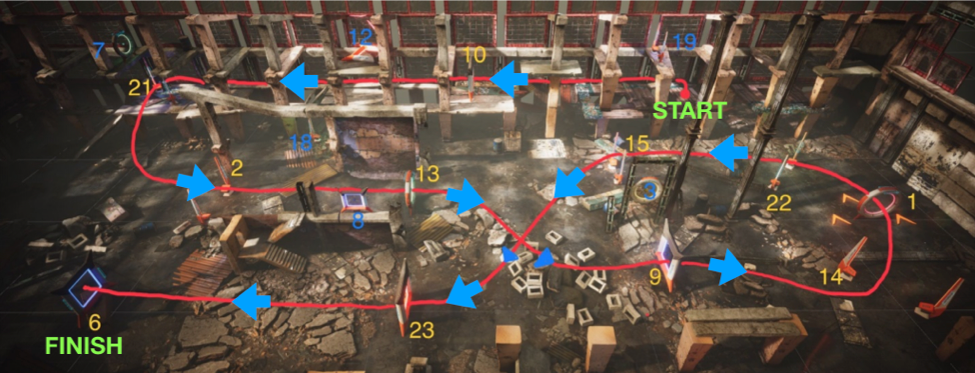
\includegraphics[width=\textwidth]{imagenes/diagramacircuito}
	\caption{Vista aérea del circuito en el simulador FightGoggles, las puertas que se deben traspasar se simbolizan con su número en color amarillo.}
	\label{waypoints:circuito}
\end{figure}

Como se puede observar en la figura \ref{waypoints:circuito} la aeronave debe recorrer 11 puertas, cada una con un número de identificación, en un orden concreto. Cada una de estas puertas posee unas medidas estandarizadas de 2x2 m.

En la competición se proporciona el orden en el que se deben atravesar las puertas y una posición aproximada de las posiciones de cada una de ellas en el mundo. Esta posición aproximada posee un error significativo, por lo que es necesario corregir la estimación de la posición de estas puertas a medida que la aeronave avanza por el circuito (estimación \textit{online}).

Para poder realizar la estimación \textit{online} de las puertas, es necesario percibirlas, para ello se hace uso de las cámaras integradas en la aeronave simulada. Las cámaras del cuadricóptero permiten localizar las distintas puertas a lo largo del circuito. La imagen provista por el simulador, además de contener la imagen observada por la cámara, contiene también las posiciones en el plano imagen, de las esquinas de las puertas visibles, así como el identificador de puerta a la que corresponde.

\tb{imagen con los puntos rojos}

Esta información extra provista por el simulador facilita enormemente la estimación de las posiciones de las distintas puertas, reduciendo también el tiempo de calculo requerido.



Dado que se cuenta con los parámetros físicos de la cámara y con las dimensiones de las puertas, es posible emplear un algoritmo PnP (\textit{Perspective n-Points}) para calcular la posición relativa de los \textit{frames} con respecto a la aeronave. Concretamente, se ha empleado la medida de la posición del centro de la puerta, ya que nos permite generar los waypoints de forma más sencilla.






La incertidumbre de estas medidas disminuye a medida que el aeronave se acerca a las puertas, por lo que cuando las imágenes se toman a una distancia lejana, el error que tienen es elevado. Para disminuir la influencia de las medidas erróneas cada medida se somete a un filtrado en dos pasos:

\begin{enumerate}
	\item \textbf{Región de confianza:} Dado que siempre se posee una posición estimada de cada puerta es posible emplear esta información para descartar medidas erróneas. Siendo $\hat{G_i}$ la estimación previa del centro de la puerta $i$, se establece una bola $B(\hat{G_i},r)$ con centro en $\hat{G_i}$  y radio $r$ como región de confianza, es decir, si una nueva medida $G_i \notin B(\hat{G_i},r)$ entonces se desecha como una medida errónea.
	El valor del radio $r$ influye en la distancia máxima que puede tener una medida respecto a la estimación original para considerarse correcta. Dado que al comienzo del circuito se tienen unas posiciones de las puertas con un error muy grande, este valor $r$ no puede ser muy bajo, si no no se conseguiría corregir la posición de las puertas con mediciones correctas. Por el contrario, si el valor de $r$ es muy grande, este filtrado carecería de sentido, ya que cualquier medición se consideraría válida. En la practica se han probado con distintos valores de este parámetro, obteniendo mejores resultados con valores de $r$ de entre 4 y 6 metros.
	\item \textbf{Media móvil:} Si la medida obtenida $G_i$ se encuentra contenida en esa región, entonces, en lugar de sustituir directamente la estimación de la posición de esta puerta, se realiza una modificación de la medición anterior, de acorde a la fórmula:
	\begin{equation}
		\hat{G_i} = \alpha \hat{G}_{i,prev} + (1-\alpha)G_i
	\end{equation}
	siendo $\hat{G}_{i,prev}$ la estimación anterior y $\alpha \in (0,1)$ un parámetro de filtrado. Cuando $\alpha$ tiene valores pequeños, la estimación cambia rápidamente con las nuevas medidas, mientras que si $\alpha$ posee valores altos, la estimación varía ligeramente con cada una de las nuevas medidas. Los valores que se suelen emplear son $\alpha = 0.9$ y $\alpha = 0.99$. Para este filtrado se ha empleado un valor de $\alpha = 0.9$ dado que presenta un buen equilibrio entre robustez y reactividad ante nuevas medidas.

\end{enumerate}

Con este proceso se consigue obtener las posiciones estimadas de las, lo que constityen 

\begin{figure}[htb!]
	\centering
	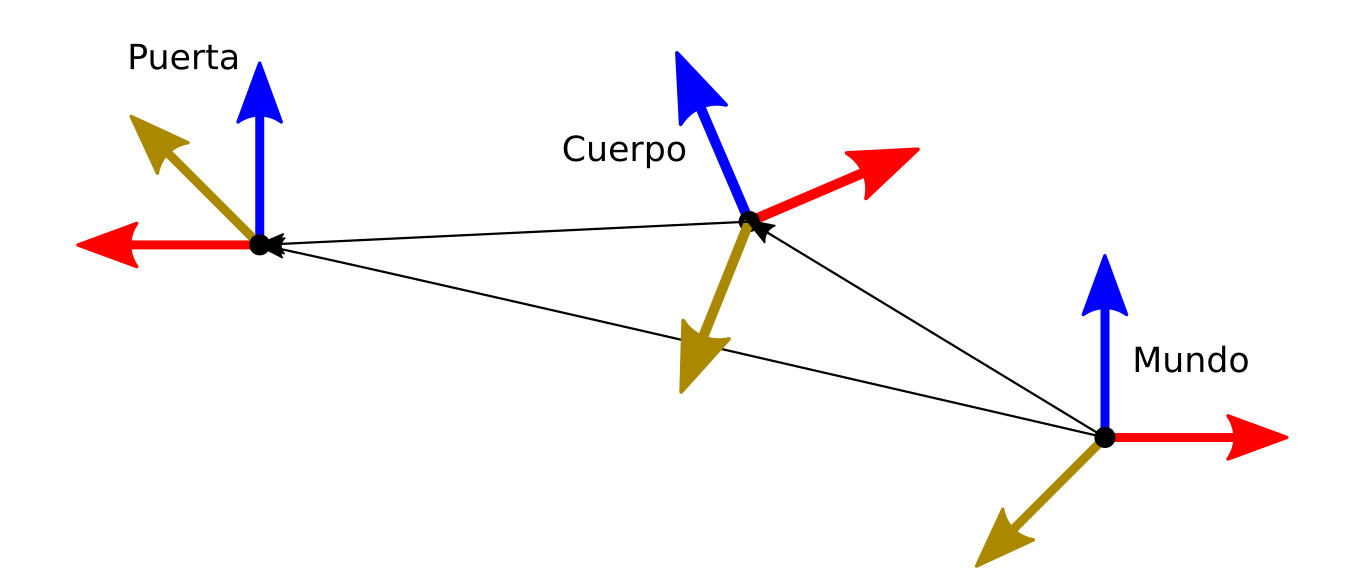
\includegraphics[width=0.75\textwidth]{imagenes/frames}
	\caption{Transformaciones entre los sistemas de referencia de las puertas, el cuerpo de la aeronave y el mundo.}
	\label{waypoints:Refs}
\end{figure}







\section{Trayectorias a largo y corto plazo}

